\documentclass[twocolumn]{article}

\usepackage{graphicx, epsfig}
\usepackage{amsmath}

\usepackage{float}

\title{Assignment 2\\Computational Physics I - Phys381}
\author{Guilherme Contesini , 10140201}


\begin{document}
\maketitle
\date{}

%%%%%%%%%%%%%%%%%%%%%%%%%%%%%%%%%%%%%%%%%%%%%%%%%%%%%%%%%%%%%%%%%%%%%%%%%%%%%%%%%%%%%%%%%%%%%%%%%%%%%%%%%%%%%%%%%%%%%%%%
\section{Introduction}
\paragraph{}
This final assignment deals with machine precision, and the limitations that computers can have regarding manipulation of numbers with infinite decimal values such as $\pi$. In the first section, we will find consider the $\pi$ approximation as a summation produced by Madhava of Sangamagrama, an Indian Mathematician. We will use both single and double precision to calculate the summation and compare it to the given value of $\pi$ which in this case, we will call:$\pi_{correct}$. For iterations up to 50, we will save the data and plot the results. 
\paragraph{}
Additionally, we will evaluate the differences between truncation error($\epsilon_{trunc.}$) and rounding error($\epsilon_{round}$). Putting the two errors together, we will find conditions for when the total error is at a minimum. 
\paragraph{}
In the second section, we examine the function: $R(r)=(2r^2-18r+27 \times exp^{-\frac{r}{3}}$ where \textit{r} is the radial component of a hydrogen electron in the 3s shell. We will again use an approximation method by means of the power series expansion. 
\paragraph{}
In the third part, the theme is LU-Decomposition(Lower-Upper-Decomposition). The method for doing this is performed in a subroutine by Crout's algorithm, found in the lecture notes. We will also examine the \textit{Condition Numbers $k_1$, $k_{\infty}$, and $k_2$}. These are important in accepting the values of the LU-Decomposition.
\paragraph{}
Lastly, we use this method to solve for acceleration of a rocket, given a 2nd degree polynomial. To approach this, we transform the polynomial into a matrix multiplication.

\emph{Note:It has been acknowledged that this assignment is very much similar to that of the requirements found in Lab #6. Therefore in fulfilling the lab requirements with my partner, we at the same time completed many of the objectives needed for Assignment #2. So similarities between our separate assignments should be expected in terms of results, methods and figures.}
%%%%%%%%%%%%%%%%%%%%%%%%%%%%%%%%%%%%%%%%%%%%%%%%%%%%%%%%%%%%%%%%%%%%%%%%%%%%%%%%%%%%%%%%%%%%%%%%%%%%%%%%%%%%%%%%%%%%%%%%
\section{Errors in computation}													
%%%%%%%%%%%%%%%%%%%%%%%%%%%%%%%%%%%%%%%%%%%%%%%%%%%%%%%%%%%%%%%%%%%%%%%%%%%%%%%%%%%%%%%%%%%%%%%%%%%%%%%%%%%%%%%%%%%%%%%%
\subsection{Calculation of $\pi$}													
%%%%%%%%%%%%%%%%%%%%%%%%%%%%%%%%%%%%%%%%%%%%%%%%%%%%%%%%%%%%%%%%%%%%%%%%%%%%%%%%%%%%%%%%%%%%%%%%%%%%%%%%%%%%%%%%%%%%%%%%
\subsubsection{-(i)}
The Fortran code can be found in the Appendix Section \ref{[Madhava algorithm]}.						
%%%%%%%%%%%%%%%%%%%%%%%%%%%%%%%%%%%%%%%%%%%%%%%%%%%%%%%%%%%%%%%%%%%%%%%%%%%%%%%%%%%%%%%%%%%%%%%%%%%%%%%%%%%%%%%%%%%%%%%%
\subsubsection{-(ii)}			
\begin{figure}[H]
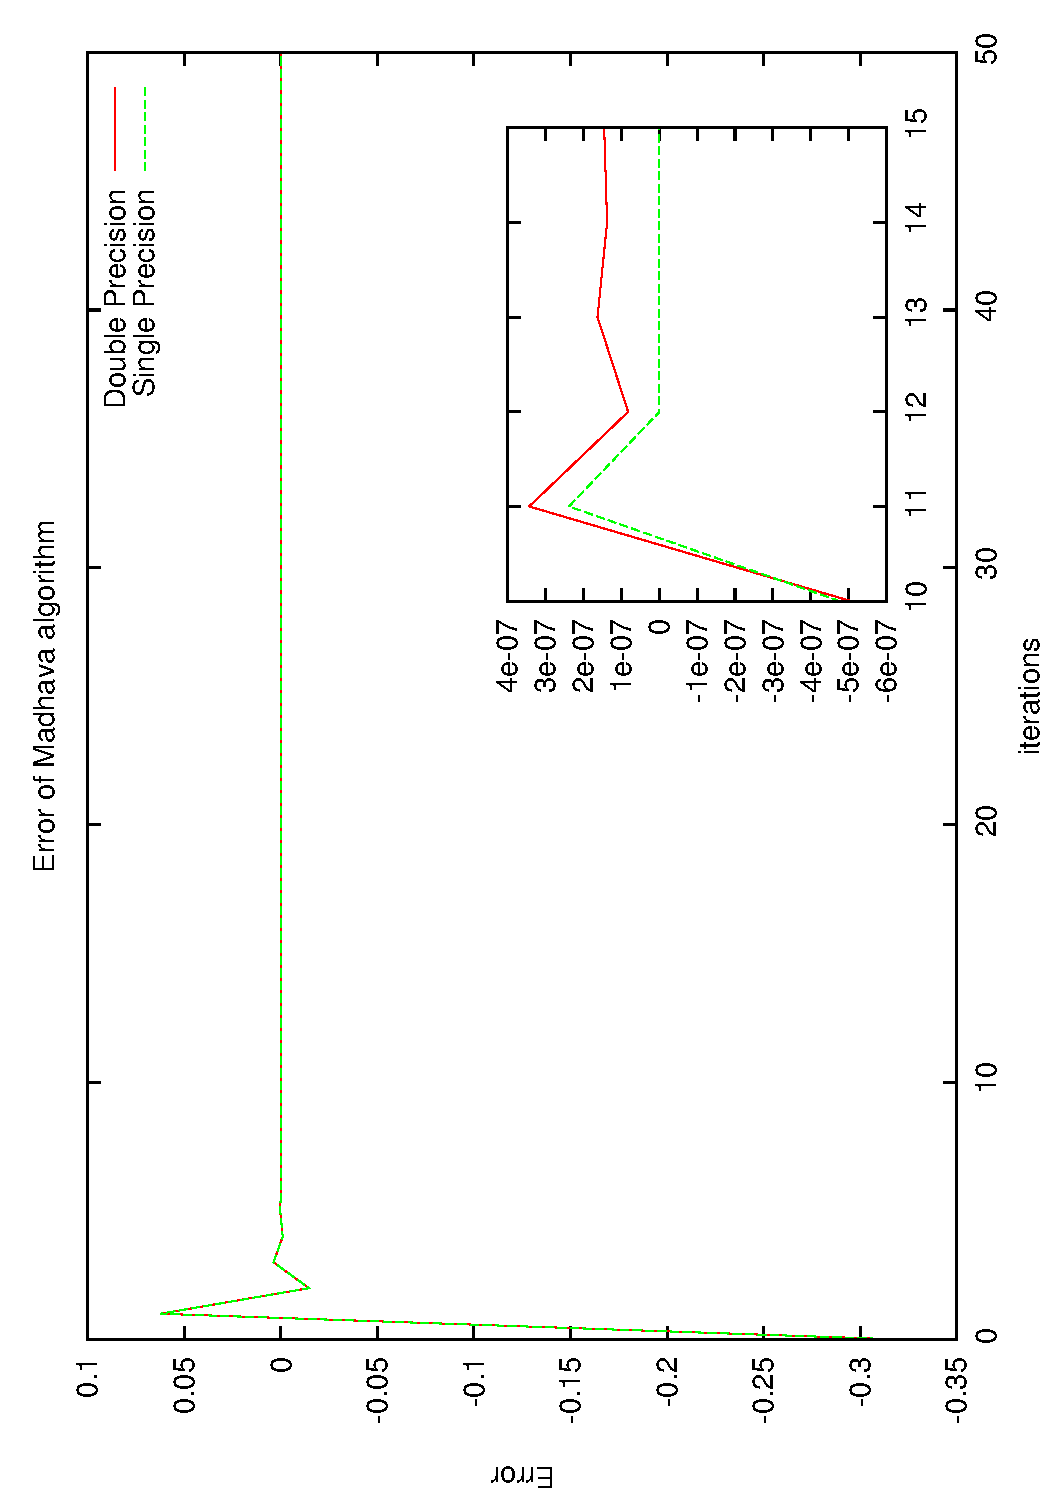
\includegraphics[width=2.in, angle=270]{ErrorofMadhavaalgorithm.pdf} 
\caption{Madhava Algorithm}\label{Madhava_Plot}
\end{figure}
gnuplot script can be found in Appendix section \ref{[Madhava gnuplot script]}.

\subsubsection{-(iii)}
Based on figure \ref{Madhava_Plot} above, it is seen that error is greatest for values $N\leq 1$. The error quickly approaches zero from $N \geq 4$. Therefore, it is reasonable to use this algorithm to estimate the value of pi for any value of N above 4.
Comparing the difference between single precision and double precision, we expected that the errors from double precision to be lower than that of single. This is true for the most part, however, when we look at figure \ref{Madhava_Plot}, double precision lies further from zero than single precision at low values of N. This may be due to the nature of having lower values of N.

%%%%%%%%%%%%%%%%%%%%%%%%%%%%%%%%%%%%%%%%%%%%%%%%%%%%%%%%%%%%%%%%%%%%%%%%%%%%%%%%%%%%%%%%%%%%%%%%%%%%%

\subsection{Error Propagation in Series Expansion}
\subsubsection*{-(i)}
To calculate for minimal $\epsilon_T$, we should take the derivative of $\epsilon_T$ with respect to the variable N, and solve for zero. From equations given to us:

\begin{subequations}
\begin{align}
\epsilon_T  &= \epsilon_{round} + \epsilon_{trunc.}\\
\epsilon_T  &= \sqrt{N} \epsilon_{m} + \frac{\alpha}{N^{\beta}}\\
\epsilon_T' &= \frac{\epsilon_m}{2 \sqrt{N}} +(-\beta)\alpha N^{(-\beta - 1)}
\end{align}
Now setting $\epsilon_T$ to zero:
\begin{align}
0 = \frac{\epsilon_m}{2 \sqrt{N}} &+(-\beta)\alpha N^{(-\beta - 1)}\\
\beta \alpha N^{(-\beta -1)} &= \frac{1}{2} N^{(-1/2)} \epsilon_m\\
\frac{2 \beta \alpha}{\epsilon_m} &= \frac{N^{(-\frac{1}{2})}}{N^{(-\beta -1)}}\\
&=N^{-\frac{1}{2} - (-\beta -1)}\\
&=N^{(-\frac{1}{2} +\beta +1)}\\
&=N^{\beta +\frac{1}{2}}
\end{align}
\end{subequations}

\subsubsection*{-(ii)}
\begin{figure}[H]
\begin{center}
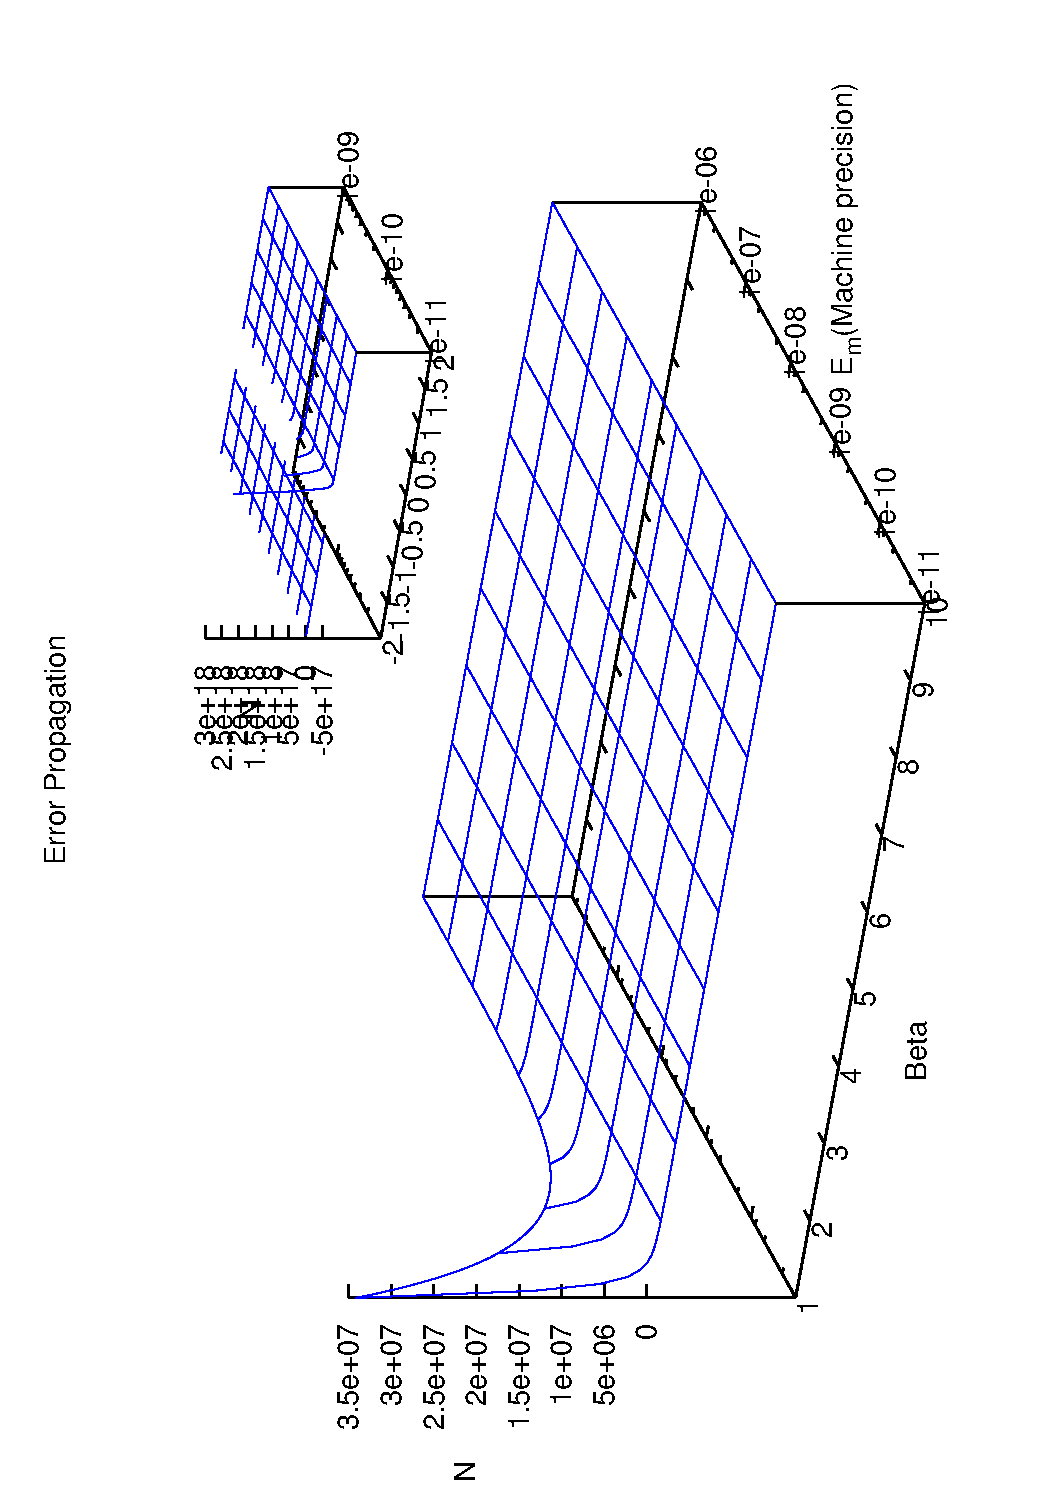
\includegraphics[width=2.0in, angle=270]{Error_propagation.pdf}
\caption{Caption}
\label{Error Propagation}
\end{center}
\end{figure}

\subsubsection*{-(iii)}
The regimes in which I would expect the round-off error to dominate over the truncated error

%%%%%%%%%%%%%%%%%%%%%%%%%%%%%%%%%%%%%%%%%%%%%%%%%%%%%%%%%%%%%%%%%%%%%%%%%%%%%%%%%%%%%%%%%%%%%%%%%%%%%

\section{Evaluation of Functions: \textit{Hydrogen Orbital Function}}
\subsection*{-(i)}
Replacing exp$^{-\frac{r}{3}}$ with the first two terms of its power series expansion, we get:
\begin{equation}
R(r) = (2r^2 - 18r +27) \times \left[1 - \frac{r}{3}\right]
\end{equation}
\subsection{-(iii)}
For small radius the a bigger series works perfect , but for large values of the radius the series expansion don't return values that matches with the reality. 
\subsection*{-(iv)}
\begin{figure}
\begin{center}
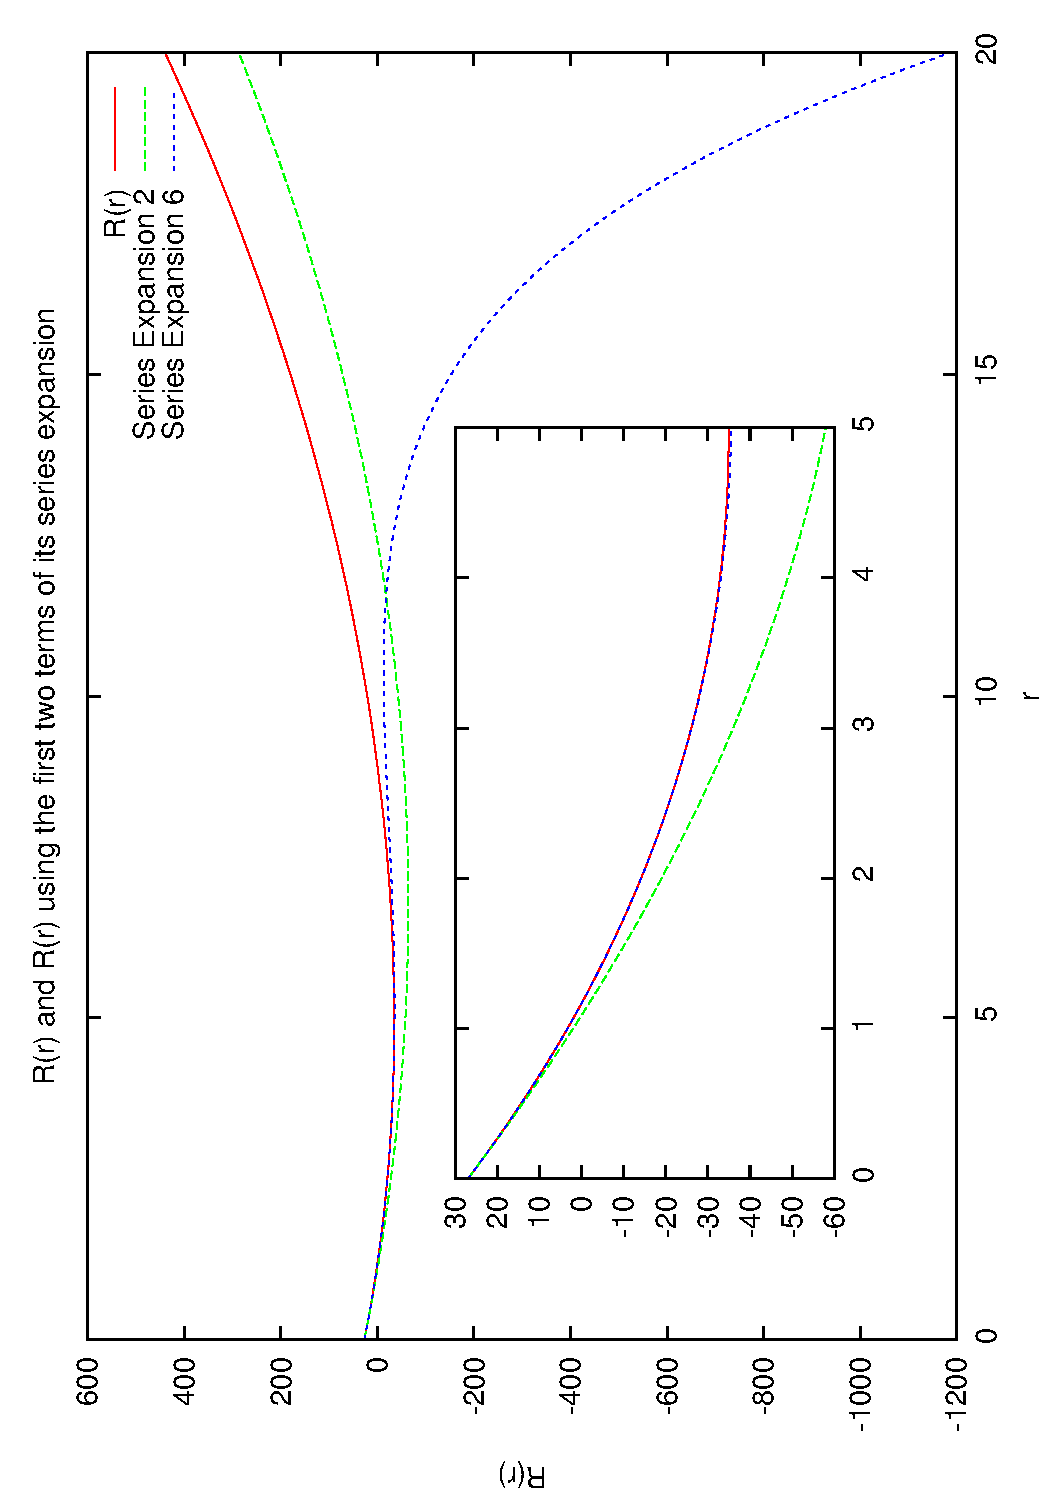
\includegraphics[width=2.0in, angle=270]{Hydrogen.pdf}
\caption{Hydrogen Orbital}
\label{Hydrogen_Orbital}
\end{center}
\end{figure}
The gnuplot script can be found in the appendix in section \ref{Hydrogen Orbital Function}.

%%%%%%%%%%%%%%%%%%%%%%%%%%%%%%%%%%%%%%%%%%%%%%%%%%%%%%%%%%%%%%%%%%%%%%%%%%%%%%%%%%%%%%%%%%%%%%%%%%%%%

\section{Matrix Algebra}
\subsection{Case A:}
\subsubsection{1-norm(k$_1$)}
k(a)$_1$ =    100001.00 \\
\newline
\subsubsection{LU-Decomposition: First set of solutions}

\begin{table}[h!]
  \centering
  \begin{tabular}{|c|c|} \hline
x & Solution\\ \hline \hline
$x_1$ & 0.99998 \\ \hline
$x_2$ & 0.99999 \\ \hline
\end{tabular}
\centering
\end{table}
\subsubsection{1-norm(k$_1$): New Condition Number}
\newline
k(a)$_1$ =    8.98
\subsubsection{LU-Decomposition: Second set of solutions}

\begin{table}[H]
  \centering
  \begin{tabular}{|c|c|} \hline
x & Solution\\ \hline \hline
$x_1$ & 199599.80 \\ \hline
$x_2$ & 99800.400 \\ \hline
\end{tabular}
\end{table}
\newline
\subsubsection{}
Its doesn't work well because the epsilon along the diagonal distorts the function.

\subsection{Case B:}
\subsubsection{LU-Decomposition: double-check solution}
\begin{table}[H]
  \centering
  \begin{tabular}{|c|c|} \hline
x & Solution\\ \hline \hline
$x_1$ & 1.00 \\ \hline
$x_2$ & 1.00 \\ \hline
$x_3$ & 1.00 \\ \hline
$x_4$ & 1.00 \\ \hline
\end{tabular}
\centering
\end{table}

\subsubsection{Small difference in the coefficient in vector B(i)}
\begin{table}[H]
  \centering
  \begin{tabular}{|c|c|} \hline
x & Solution\\ \hline \hline
$x_1$ & -7.199 \\ \hline
$x_2$ &  5.999 \\ \hline
$x_3$ & 2.899  \\ \hline
$x_4$ & -9.999E-002 \\ \hline
\end{tabular}
\centering
\end{table}

\subsubsection{Slight change to the coefficient in vector B(ii)}
\begin{table}[H]
  \centering
  \begin{tabular}{|c|c|} \hline
x & Solution\\ \hline \hline
$x_1$ & 1.710 \\ \hline
$x_2$ & 0.599 \\ \hline
$x_3$ & 0.739 \\ \hline
$x_4$ & 1.160 \\ \hline
\end{tabular}
\centering
\end{table}
\subsubsection{Condition Number $k_{inf}$}
k(a)inf =    4487.9999999998199

%%%%%%%%%%%%%%%%%%%%%%%%%%%%%%%%%%%%%%%%%%%%%%%%%%%%%%%%%%%%%%%%%%%%%%%%%%%%%%%%%%%%%%%%%%%%%%%%%%%%%
\subsection{Rocket Physics}
\subsubsection{Linear System: Ax =B}

\begin{bmatrix}
$t^2$ & t & 1
\end{bmatrix}
$\times$
\begin{bmatrix}
$a_1$ \\
$a_2$ \\
$a_3$ \\
\end{bmatrix}
=
\begin{bmatrix}
$v(t)$
\end{bmatrix}

\subsubsection{}
The Fortran Code for Gauss can be found at section \ref{Gauss}, and LU Decomposition code can be found at section \ref{LU Decomposition2}

\subsubsection{Gauss Solution}

\begin{table}[H]
  \centering
  \begin{tabular}{|c|c|} \hline
x & Solution\\ \hline \hline
$a_1$ & 0.290477026076542 \\ \hline
$a_2$ & 19.6904632931664  \\ \hline
$a_3$ & 1.08576093401218 \\ \hline
\end{tabular}
\centering
\end{table}

\subsubsection{LU Decomposition Solution}
\begin{table}[H]
  \centering
  \begin{tabular}{|c|c|} \hline
x & Solution\\ \hline \hline
$a_1$ & 0.290477026076 \\ \hline
$a_2$ & 19.69046329316  \\ \hline
$a_3$ & 1.085760934012 \\ \hline
\end{tabular}
\centering
\end{table}
  
\subsubsection{}
\begin{table}[H]
  \centering
  \begin{tabular}{|c|c|} \hline
x & Solution\\ \hline \hline
t=6 & 129.66500294208527 \\ \hline
t=7.5 & 165.07250357419252 \\ \hline
t=9 & 201.78500416874886  \\ \hline
t=15 & 361.68500617146492 \\ \hline
\end{tabular}
\centering
\end{table}

%%%%%%%%%%%%%%%%%%%%%%%%%%%%%%%%%%%%%%%%%%%%%%%%%%%%%%%%%%%%%%%%%%%%%%%%%%%%%%%%%%%%%%%%%%%%%%%%%%%%%


\section{Conclusion}
We have now covered all of the information we need with regards to precision and error in completion of this assignment. We are now well aware of what limitations our computers have and their respective consequences. In the latter portion of this assignment, we explored the method of LU-Decomposition. This is a quick and easy way to solve for a single vector in the system of [Ax = B] where A and B are Matrices of size nxn, and x is a column vector size n. Generally, this procedure is an algorithm in which each array cell is solved and used to solve the next line. This only possible when we transform the matrices into lower and upper matrices, where the values are zero above the diagonal and below the diagonal respectively.

%%%%%%%%%%%%%%%%%%%%%%%%%%%%%%%%%%%%%%%%%%%%%%%%%%%%%%%%%%%%%%%%%%%%%%%%%%%%%%%%%%%%%%%%%%%%%%%%%%%%%
%%%%%%%%%%%%%%%%%%%%%%%%%%%%%%%%%%%%%%%%%%%%%%%%%%%%%%%%%%%%%%%%%%%%%%%%%%%%%%%%%%%%%%%%%%%%%%%%%%%%%
%%%%%%%%%%%%%%%%%%%%%%%%%%%%%%%%%%%%%%%%%%%%%%%%%%%%%%%%%%%%%%%%%%%%%%%%%%%%%%%%%%%%%%%%%%%%%%%%%%%%%
\section{Appendix Codes:}
%%%%%%%%%%%%%%%%%%%%%%%%%%%%%%%%%%%%%%%%%%%%%%%%%%%%%%%%%%%%%%%%%%%%%%%%%%%%%%%%%%%%%%%%%%%%%%%%%%%%%%%%%%%%%%%%%%%%%%%%
\subsection{Madhava algorithm-(i)}\label{[Madhava algorithm]}
\begin{verbatim}
program indian_pi
  implicit none
  double precision :: my_pi_dp , 
  real_pi_dp , sum_dp , pi_dp
  real :: sum_float , my_pi_float , 
pi_float
  integer :: i_int
  open(12,file="pi_error.txt",action=
"write")
  pi_dp = 3.141592653589793
  pi_float = 3.141592653589793
  sum_dp = 0.
  sum_float = 0.
  do i_int = 0,50,1
    sum_dp = (((-1.)**(i_int))/(((2.*
    i_int)+1)*(3.**i_int))) + sum_dp
    sum_float = (((-1.)**(i_int))/
    (((2.*i_int)+1)*(3.**i_int))) 
    + sum_float
    my_pi_dp = sqrt(12.)*sum_dp
    my_pi_float = sqrt(12.)*sum_float
    write(12,*)i_int , (pi_float-
    my_pi_float) , (pi_dp-my_pi_dp)
  end do
  close(12)
end program
\end{verbatim}
%%%%%%%%%%%%%%%%%%%%%%%%%%%%%%%%%%%%%%%%%%%%%%%%%%%%%%%%%%%%%%%%%%%%%%%%%%%%%%%%%%%%%%%%%%%%%%%%%%%%%%%%%%%%%%%%%%%%%%%%
\subsection{Gnuplot Script for Madhava Algorithm-(ii)} \label{[Madhava gnuplot script]}
\begin{verbatim}
reset
set terminal postscript color enhanced 
set output "ErrorofMadhavaalgorithm.eps"
set size 1,1
set origin 0,0
set multiplot
set title 'Error of Madhava algorithm'
set xlabel 'iterations'
set ylabel 'Error'
set xrange [0:50]
plot 'pi_error.txt' u 1:3 w l title 
	 'Double Precision',\
     'pi_error.txt' u 1:2 w l title
     'Single Precision'
unset key
unset xlabel
unset ylabel
unset title
set xrange [10:15]
set origin 0.50,0.1
set size 0.45,0.45
replot
!epstopdf "ErrorofMadhavaalgorithm.eps"
 && rm "ErrorofMadhavaalgorithm.eps"
reset
\end{verbatim}

\subsection{3D Error Propagation Plot}\label{3D Error Plot}
\begin{verbatim}
reset
set terminal postscript color enhanced 
set output"Error_propagation.eps"
f(x,y)=((2*a*x/y))**(1/(x+0.5))
a=1
set title 'Error Propagation'
set xlabel 'Beta'
set ylabel 'E_m(Machine precision)'
set zlabel 'N'
set xrange[1:10]
set yrange[10.e-12:10e-7]
set logscale y
set size 1,1
set origin 0,0
set multiplot
splot f(x,y) linecolor rgb "blue" notitle
unset key
unset xlabel
unset ylabel
unset title
set xrange[-2:2]
set yrange[1e-11:1e-9]
set origin 0.5,0.5
set size 0.45,0.45
replot 
!epstopdf "Error_propagation.eps" &&
 rm "Error_propagation.eps"
reset
\end{verbatim}
\subsection{Evaluation of Function}\label{Hydrogen Orbital Function}
\begin{verbatim} 
reset
set terminal postscript color enhanced 
set output"Hydrogen.eps" 
set multiplot 
set title 'R(r) and R(r) using the 
first two terms of its series expansion' 
set xlabel 'r' 
set ylabel 'R(r)' 
set xrange[0:20] 
set size 1,1
set origin 0,0

g(x)=(2.*x**2-18.*x+27.*exp(-x/3.)) 
f(x)=(2.*x**2-18.*x+27.*(1.-(x/3.)))
h(x)=(2.*x**2.-18.*x+27.*(1.-(x/3.)+
(x**2./18.)-(x**3./162.)+(x**4./1944.)-
(x**5./29160.)))

plot g(x) title "R(r)",\
     f(x) title "Series Expansion 2",\
     h(x) title "Series Expansion 6"

unset key
unset xlabel
unset ylabel
unset title
set xrange[0:5]
set origin 0.15,0.15
set size 0.6,0.45
replot 

!epstopdf "Hydrogen.eps" && 
 rm "Hydrogen.eps"
reset

\end{verbatim}
\subsection{Matrix Algebra}\label{LU Decomposition1}
\begin{verbatim}
program LU_decomposition
  implicit none
  integer :: size_int
  double precision , dimension(3,3) 
  :: L_mtx , U_mtx , a_mtx , b_vec
  double precision , dimension(3,3) 
  :: aux_vec, sol_vec , inv_a_mtx , 
  inv_a_vec
  double precision :: norm_1_dp,
 norm_inf_dp, norm_2_dp,
 norm_inv_1_dp, norm_inv_inf_dp,
 norm_inv_2_dp, k_a_1_dp, k_inf_dp
  size_int = 3
  a_mtx(1,1) = 5
  a_mtx(1,2) = 7
  a_mtx(1,3) = 6
  a_mtx(1,4) = 5
  a_mtx(2,1) = 7
  a_mtx(2,2) = 1
  a_mtx(2,3) = 8
  a_mtx(2,4) = 7
  a_mtx(3,1) = 6
  a_mtx(3,2) = 8
  a_mtx(3,3) = 10
  a_mtx(3,4) = 9
  a_mtx(4,1) = 5
  a_mtx(4,2) = 7
  a_mtx(4,3) = 9
  a_mtx(4,4) = 10
  b_vec(1,1) = 1
  b_vec(2,1) = 1
  b_vec(3,1) = 1
  b_vec(4,1) = 1
  call clean_matrix(L_mtx,size_int)
  call clean_matrix(U_mtx,size_int)
  call clean_matrix(sol_vec,size_int)
  call clean_matrix(aux_vec,size_int)
  call clean_matrix(inv_a_vec,size_int)
  call clean_matrix(inv_a_mtx,size_int)
  call LUdecompCrout(a_mtx,L_mtx,
  U_mtx,size_int)
  call ProgresSub(L_mtx,b_vec,
  aux_vec,size_int)
  call RegresSub(U_mtx,aux_vec,
  sol_vec,size_int)
  call inverse(inv_a_mtx,a_mtx,
  size_int)
  write(*,*) ""
  write(*,*) "Solution"
  write(*,*) ""
  call print_vector(sol_vec,size_int)
  write(*,*) ""
  write(*,*) ""
  write(*,*) "inverse"
  write(*,*) ""
  call print_matrix(inv_a_mtx,size_int)
  write(*,*) ""
  norm_1_dp = MAXVAL(SUM(ABS(
  a_mtx),DIM=1))
  norm_inf_dp = MAXVAL(SUM(ABS(
  a_mtx),DIM=2))
  norm_2_dp = SQRT(SUM(a_mtx**2.0))
  write(*,*) 'norm_1 = ', norm_1_dp
  write(*,*) 'norm_inf = ', norm_inf_dp
  write(*,*) 'norm_2 = ', norm_2_dp
  write(*,*) ""
  norm_inv_1_dp = MAXVAL(SUM(ABS(
  inv_a_mtx),DIM=1))
  norm_inv_inf_dp = MAXVAL(SUM(ABS(
  inv_a_mtx),DIM=2))
  norm_inv_2_dp = SQRT(SUM(inv_a_mtx**2.0))
  write(*,*) 'norm_1 = ', norm_inv_1_dp
  write(*,*) 'norm_inf = ', norm_inv_inf_dp
  write(*,*) 'norm_2 = ', norm_inv_2_dp
  write(*,*) ""
  k_a_1_dp = norm_1_dp * norm_inv_1_dp
  k_inf_dp = norm_inf_dp * norm_inv_inf_dp
  write(*,*) 'k(a)1 = ' , k_a_1_dp
  write(*,*) 'k(a)inf = ' , k_inf_dp

contains

subroutine clean_matrix(a_mtx,size_int)
  implicit none
  integer , intent(in) :: size_int
  double precision , intent(out) , 
dimension(size_int,size_int) :: a_mtx
  integer :: i_int , j_int
  do i_int = 1, size_int
    do j_int = 1,size_int
      a_mtx(i_int,j_int) = 0
    end do 
  end do
end subroutine

subroutine LUdecompCrout(a_mtx,L_mtx,
  U_mtx,size_int) 
  implicit none
  integer , intent(in) :: size_int
  double precision , intent(in) , 
  dimension(size_int,size_int) :: a_mtx
  double precision , intent(out) , 
  dimension(size_int,size_int) :: 
  L_mtx , U_mtx
  integer :: i_int , j_int , k_int
  double precision :: sum_float
  !step 1 & 2
  do i_int = 1,size_int,1
    L_mtx(i_int,1) = a_mtx(i_int,1)
    U_mtx(i_int,i_int) = 1.
  end do
  !step 3
  do j_int = 2,size_int,1
    U_mtx(1,j_int) = a_mtx(1,j_int)
    /L_mtx(1,1)
  end do 
  !step 4
  do i_int=2,size_int
    do j_int=2,i_int
      sum_float = 0.
      do k_int=1,j_int-1,1
        sum_float = sum_float + 
  L_mtx(i_int,k_int)*U_mtx(k_int,j_int)
      end do
      L_mtx(i_int,j_int) = a_mtx(i_int
  ,j_int) - sum_float
    end do
    do j_int=i_int+1,size_int,1
      sum_float = 0.
      do k_int = 1,i_int-1,1
        sum_float = sum_float + 
  L_mtx(i_int,k_int)*U_mtx(k_int,j_int)
      end do
      U_mtx(i_int,j_int) = (a_mtx(i_int
  ,j_int)-sum_float)/L_mtx(i_int,i_int)
    end do
  end do
end subroutine

subroutine ProgresSub(a_mtx,b_vec,
  aux_vec,size_int)
  implicit none
  integer , intent(in) :: size_int
  double precision , intent(in) , 
dimension(size_int,size_int) :: a_mtx
  double precision , intent(in) , 
  dimension(size_int,1) :: b_vec
  double precision , intent(out) , 
  dimension(size_int,1) :: aux_vec
  integer :: i_int , j_int
  double precision :: sum_float
  aux_vec(1,1) = b_vec(1,1)/a_mtx(1,1)
  do i_int=2,size_int
    sum_float = 0.
    do j_int = 1,i_int-1,1
      sum_float = sum_float + (a_mtx(
  i_int,j_int)*aux_vec(j_int,1))
    end do
    aux_vec(i_int,1) = (b_vec(i_int,1
  )-sum_float)/a_mtx(i_int,i_int)
  end do
end subroutine

subroutine RegresSub(a_mtx,b_vec,
  sol_vec,size_int)
  implicit none
  integer , intent(in) :: size_int
  double precision , intent(in) ,
  dimension(size_int,size_int) :: a_mtx
  double precision , intent(in) , 
  dimension(size_int,1) :: b_vec
  double precision , intent(out) ,
  dimension(size_int,1) :: sol_vec
  integer :: i_int , j_int
  double precision :: sum_float
  sol_vec(size_int,1) = b_vec(size_int,
  1)/a_mtx(size_int,size_int)
  do i_int = size_int-1,1,-1
    sum_float = 0.
    do j_int =size_int,i_int+1,-1
      sum_float = sum_float + a_mtx(
  i_int,j_int )*sol_vec(j_int,1)
    end do
    sol_vec(i_int,1) = ( b_vec(i_int,
  1) - sum_float )/a_mtx(i_int,i_int)
  end do
end subroutine

subroutine print_matrix(s_mtx,size_int)
  implicit none
  integer , intent(in) :: size_int
  double precision , intent(in) , 
  dimension(size_int,size_int) :: s_mtx
  integer :: i_int , j_int
  do i_int=1,size_int
    do j_int=1,size_int
      if(j_int==size_int) then
        write(*,"(f9.4)",advance="yes")
  s_mtx(i_int,j_int)
      else
        write(*,"(f9.4)",advance="no")
  s_mtx(i_int,j_int)
      end if
    end do
  end do 
end subroutine

subroutine inverse(inv_a_mtx,a_mtx,size_int)
  implicit none
  integer , intent(in) :: size_int
  double precision, intent(in) , 
  dimension(size_int,size_int) :: a_mtx 
  double precision , intent(out) , 
  dimension(size_int, size_int) :: 
  inv_a_mtx 
  double precision , dimension(size_int
  ,size_int) :: L_mtx ,U_mtx, i_mtx ,
   i_vec
  double precision , dimension(size_int
  ,size_int) :: aux_vec , sol_vec
  integer :: i_int , j_int
  call clean_matrix(L_mtx,size_int)
  call clean_matrix(U_mtx,size_int)
  call clean_matrix(sol_vec,size_int)
  call clean_matrix(aux_vec,size_int)
  call clean_matrix(i_vec,size_int)
  call identity(i_mtx,size_int)
  do i_int = 1 , size_int
    do j_int = 1, size_int
      i_vec(j_int,1) = i_mtx(j_int,i_int)
    end do
    call LUdecompCrout(a_mtx,L_mtx,
  U_mtx,size_int)
    call ProgresSub(L_mtx,i_vec,
  aux_vec,size_int)
    call RegresSub(U_mtx,aux_vec,
  sol_vec,size_int)
    do j_int = 1, size_int
      inv_a_mtx(j_int,i_int) = 
  sol_vec(j_int,1)
    end do 
  end do
end subroutine

subroutine identity(i_mtx,size_int)
  implicit none
  integer , intent(in) :: size_int
  double precision , intent(out) , 
dimension(size_int,size_int) :: i_mtx
  integer :: i_int , j_int
  do i_int = 1,size_int
    do j_int = 1, size_int
      i_mtx(i_int,j_int) = 0
    end do 
    i_mtx(i_int,i_int) = 1
  end do 
end subroutine

subroutine print_vector(s_vec,size_int)
  implicit none
  integer , intent(in) :: size_int
  double precision , intent(in) , 
  dimension(size_int,size_int) :: s_vec
  integer :: i_int
  do i_int=1,size_int
      write(*,"(f9.2)",advance="yes")
  s_vec(i_int,1)
  end do 
end subroutine

end program
\end{verbatim}
\subsection{Gauss Algorithm} \label{Gauss}
\begin{verbatim}
program Gauss
implicit none
integer :: size_int
double precision ,  dimension(3,3) :: a_mtx
 , x_vec , b_vec 
size_int = 3
a_mtx(1,1) = 25
a_mtx(1,2) = 5
a_mtx(1,3) = 1
b_vec(1,1) = 106.8
  call clean_matrix(x_vec,size_int)
  call gauss_elimination( a_mtx,
b_vec,size_int )
  call RegresSub(a_mtx,b_vec,x_vec,size_int)
  write(*,*) ""
  write(*,*) "Solution"
  write(*,*) ""
  call print_vector(x_vec,size_int)

contains 

subroutine gauss_elimination
( a_mtx,b_vec,size_int )
  implicit none
  integer , intent(in) :: size_int
  double precision , intent(out) ,
 dimension(size_int,size_int) :: a_mtx ,
 b_vec
  integer :: i_int , j_int , k_int
  double precision :: coef_dp 
  do i_int = 1,size_int -1
  do j_int = i_int+1,size_int
    coef_dp = a_mtx(j_int,i_int)/
a_mtx(i_int,i_int)
  do k_int = i_int , size_int
    a_mtx(j_int,k_int) = 
(a_mtx(j_int,k_int)-a_mtx
(i_int,k_int)*coef_dp  )
  end do
    b_vec(j_int,1) = ( b_vec(j_int,1)-
b_vec(i_int,1)*coef_dp  )
  end do
  end do
end subroutine

subroutine RegresSub(a_mtx,b_vec,sol_vec
,size_int)
  implicit none
  integer , intent(in) :: size_int
  double precision , intent(in) ,
 dimension(size_int,size_int) :: a_mtx
  double precision , intent(in) ,
 dimension(size_int,1) :: b_vec
  double precision , intent(out) ,
 dimension(size_int,1) :: sol_vec
  integer :: i_int , j_int
  double precision :: sum_float
  sol_vec(size_int,1) = b_vec(size_int,1)/
a_mtx(size_int,size_int)
  do i_int = size_int-1,1,-1
    sum_float = 0.
    do j_int =size_int,i_int+1,-1
      sum_float = sum_float + 
      a_mtx(i_int,j_int )*
sol_vec(j_int,1)
    end do
    sol_vec(i_int,1) = ( b_vec(i_int,1)
     - sum_float )
/a_mtx(i_int,i_int)
  end do
end subroutine

  subroutine print_matrix(a_mtx,size_int)
    implicit none
    integer , intent(in) :: size_int 
    double precision , intent(in) , 
    dimension
(size_int,size_int) :: a_mtx
    integer :: i_int , j_int
    do i_int=1,size_int
      do j_int=1,size_int
        if(j_int==size_int) then
          write(*,"(f6.2)",advance="yes")
           a_mtx(i_int,j_int)
        else
          write(*,"(f6.2)",advance="no")
           a_mtx(i_int,j_int)
        end if
      end do
    end do 
  end subroutine

  subroutine print_vector(s_vec,size_int)
    implicit none
    integer , intent(in) :: size_int
    double precision , intent(in) , 
    dimension(size_int,size_int) :: s_vec
    integer :: i_int
    do i_int=1,size_int
        write(*,"(f9.2)",advance="yes")
        s_vec(i_int,1)
    end do 
  end subroutine

subroutine clean_matrix(a_mtx,size_int)
  implicit none
  integer , intent(in) :: size_int
  double precision , intent(out) , 
  dimension(size_int,size_int) :: a_mtx
  integer :: i_int , j_int
  do i_int = 1, size_int
    do j_int = 1,size_int
      a_mtx(i_int,j_int) = 0
    end do 
  end do
end subroutine

end program
\end{verbatim}

\subsection{LU Decomposition} \label{LU Decomposition2}
\begin{verbatim}
program LU_decomposition
  implicit none
  integer :: size_int
  double precision , dimension(3,3) :: 
  L_mtx , U_mtx , a_mtx , b_vec , sol_vec
  , aux_vec
  size_int = 2
  a_mtx(1,1) = 25
  a_mtx(1,2) = 5
  a_mtx(1,3) = 1
  b_vec(1,1) = 106.8
  call clean_matrix(L_mtx,size_int)
  call clean_matrix(U_mtx,size_int)
  call clean_matrix(sol_vec,size_int)
  call clean_matrix(aux_vec,size_int)
  call LUdecompCrout(a_mtx,L_mtx,U_mtx
  ,size_int)
  call ProgresSub(L_mtx,b_vec,aux_vec
  ,size_int)
  call RegresSub(U_mtx,aux_vec,sol_vec
  ,size_int)
  write(*,*) ""
  write(*,*) "Solution"
  write(*,*) ""
  call print_vector(sol_vec,size_int)
  write(*,*) ""

contains

subroutine clean_matrix(a_mtx,size_int)
  implicit none
  integer , intent(in) :: size_int
  double precision , intent(out) , 
  dimension(size_int,size_int) :: a_mtx
  integer :: i_int , j_int
  do i_int = 1, size_int
    do j_int = 1,size_int
      a_mtx(i_int,j_int) = 0
    end do 
  end do
end subroutine

subroutine LUdecompCrout(a_mtx,L_mtx,
U_mtx,size_int) 
  implicit none
  integer , intent(in) :: size_int
  double precision , intent(in) ,
 dimension(size_int,size_int) :: a_mtx
  double precision , intent(out) ,
 dimension(size_int,size_int) :: L_mtx ,
  U_mtx
  integer :: i_int , j_int , k_int
  double precision :: sum_float
  !step 1 & 2
  do i_int = 1,size_int,1
    L_mtx(i_int,1) = a_mtx(i_int,1)
    U_mtx(i_int,i_int) = 1.
  end do
  !step 3
  do j_int = 2,size_int,1
    U_mtx(1,j_int) = 
    a_mtx(1,j_int)/L_mtx(1,1)
  end do 
  !step 4
  do i_int=2,size_int
    do j_int=2,i_int
      sum_float = 0.
      do k_int=1,j_int-1,1
        sum_float = sum_float + 
        L_mtx(i_int,k_int)
*U_mtx(k_int,j_int)
      end do
      L_mtx(i_int,j_int) = 
      a_mtx(i_int,j_int) - sum_float
    end do
    do j_int=i_int+1,size_int,1
      sum_float = 0.
      do k_int = 1,i_int-1,1
        sum_float = sum_float + 
        L_mtx(i_int,k_int)
*U_mtx(k_int,j_int)
      end do
      U_mtx(i_int,j_int) = 
      (a_mtx(i_int,j_int)-
      sum_float)/L_mtx(i_int,i_int)
    end do
  end do
end subroutine

subroutine ProgresSub(a_mtx,b_vec,
aux_vec,size_int)
  implicit none
  integer , intent(in) :: size_int
  double precision , intent(in) , 
  dimension(size_int,size_int) :: a_mtx
  double precision , intent(in) , 
  dimension(size_int,1) :: b_vec
  double precision , intent(out) , 
  dimension(size_int,1) :: aux_vec
  integer :: i_int , j_int
  double precision :: sum_float
  aux_vec(1,1) = b_vec(1,1)/a_mtx(1,1)
  do i_int=2,size_int
    sum_float = 0.
    do j_int = 1,i_int-1,1
      sum_float = sum_float + 
      (a_mtx(i_int,j_int)
	  *aux_vec(j_int,1))
    end do
    aux_vec(i_int,1) = 
    (b_vec(i_int,1)-sum_float)
/a_mtx(i_int,i_int)
  end do
end subroutine

subroutine RegresSub(a_mtx,b_vec,
sol_vec,size_int)
  implicit none
  integer , intent(in) :: size_int
  double precision , intent(in) , 
  dimension(size_int,size_int) :: a_mtx
  double precision , intent(in) , 
  dimension(size_int,1) :: b_vec
  double precision , intent(out) , 
  dimension(size_int,1) :: sol_vec
  integer :: i_int , j_int
  double precision :: sum_float
  sol_vec(size_int,1) = 
  b_vec(size_int,1)/a_mtx
(size_int,size_int)
  do i_int = size_int-1,1,-1
    sum_float = 0.
    do j_int =size_int,i_int+1,-1
      sum_float = sum_float + 
      a_mtx(i_int,j_int )*
      sol_vec(j_int,1)
    end do
    sol_vec(i_int,1) = 
    ( b_vec(i_int,1) - sum_float )
/a_mtx(i_int,i_int)
  end do
end subroutine

subroutine print_matrix(s_mtx,size_int)
  implicit none
  integer , intent(in) :: size_int
  double precision , intent(in) , 
  dimension(size_int,size_int) :: s_mtx
  integer :: i_int , j_int
  do i_int=1,size_int
    do j_int=1,size_int
      if(j_int==size_int) then
        write(*,"(f9.2)",advance="yes") 
        s_mtx(i_int,j_int)
      else
        write(*,"(f9.2)",advance="no")
         s_mtx(i_int,j_int)
      end if
    end do
  end do 
end subroutine

subroutine print_vector(s_vec,size_int)
  implicit none
  integer , intent(in) :: size_int
  double precision , intent(in) , 
  dimension(size_int,size_int) :: s_vec
  integer :: i_int
  do i_int=1,size_int
      write(*,"(f9.2)",advance="yes")
      s_vec(i_int,1)
  end do 
end subroutine

end program
\end{verbatim}
\end{document}